%% =============================================================
%%  Network Intrusion Detection System — Modern A0 Poster
%%  pdflatex — Overleaf & MiKTeX compatible
%% =============================================================
\documentclass{article}

\usepackage[paperwidth=594mm, paperheight=841mm,
            top=12mm, bottom=12mm, left=12mm, right=12mm]{geometry}
\usepackage[utf8]{inputenc}
\usepackage[T1]{fontenc}
\usepackage{helvet}
\renewcommand{\familydefault}{\sfdefault}
\usepackage{microtype}
\usepackage{xcolor}
\usepackage[most]{tcolorbox}
\usepackage{tikz}
\usetikzlibrary{shapes.geometric,arrows.meta,calc,backgrounds}
\usepackage{pgfplots}
\pgfplotsset{compat=1.18}
\usepackage{booktabs}
\usepackage{array}
\usepackage{colortbl}
\usepackage{enumitem}
\usepackage{amsmath}
\usepackage{amssymb}
\usepackage{fontawesome5}

\tikzset{>=Stealth}
\pagestyle{empty}
\setlength{\parindent}{0pt}
\setlength{\parskip}{0pt}

%% =============================================================
%%  COLOR PALETTE (COHESIVE BLUE IDENTITY)
%% =============================================================
\definecolor{Primary}{HTML}{1E3A8A}      % Blue 900 (Main theme)
\definecolor{Secondary}{HTML}{2563EB}    % Blue 600 (Accents)
\definecolor{Accent}{HTML}{38BDF8}       % Sky 400 (Highlights)
\definecolor{Background}{HTML}{F8FAFC}   % Slate 50 (Poster BG)
\definecolor{BoxBG}{HTML}{FFFFFF}        % White (Box BG)
\definecolor{TextMain}{HTML}{0F172A}     % Slate 900 (Main text)
\definecolor{TextMuted}{HTML}{475569}    % Slate 600 (Muted text)
\definecolor{BorderColor}{HTML}{E2E8F0}  % Slate 200 (Borders)
\definecolor{HighlightBG}{HTML}{F1F5F9}  % Slate 100 (Table rows)

%% Specific colors for classes (kept subtle so they don't break identity)
\definecolor{NormalColor}{HTML}{10B981}  % Emerald
\definecolor{DosColor}{HTML}{EF4444}     % Red
\definecolor{ProbeColor}{HTML}{F59E0B}   % Amber
\definecolor{R2LColor}{HTML}{8B5CF6}     % Purple
\definecolor{U2RColor}{HTML}{EC4899}     % Pink

%% =============================================================
%%  DIMENSIONS
%%  Total width = 594. Margins = 12+12=24. Usable = 570.
%%  3 Columns: 3 * 180mm = 540mm. Gaps: 2 * 15mm = 30mm.
%% =============================================================
\newlength{\colW}  \setlength{\colW}{180mm}
\newlength{\gapW}  \setlength{\gapW}{15mm}

%% =============================================================
%%  FONT SHORTCUTS
%% =============================================================
\newcommand{\sectionfont}{\fontsize{19}{23}\selectfont\bfseries}
\newcommand{\bodyfont}{\fontsize{16}{22}\selectfont}
\newcommand{\smallfont}{\fontsize{14}{19}\selectfont}
\newcommand{\tinyfont}{\fontsize{12}{15}\selectfont}
\newcommand{\metricfont}{\fontsize{36}{42}\selectfont\bfseries}
\newcommand{\labelfont}{\fontsize{14}{18}\selectfont\bfseries}

%% Colored caret bullet
\newcommand{\citem}[1]{\item[\textcolor{Secondary}{\faCaretRight}] #1}
\newcommand{\citembold}[1]{\item[\textcolor{Secondary}{\faCaretRight}] \textbf{#1}}

%% =============================================================
%%  TCOLORBOX PRESETS
%% =============================================================
\tcbset{
  pc/.style={
    enhanced, arc=6mm,
    colback=BoxBG, colframe=BorderColor,
    boxrule=1.5pt, drop fuzzy shadow=black!5!white,
    left=6mm, right=6mm, top=14mm, bottom=6mm,
    fonttitle=\sectionfont, coltitle=white, valign=top,
    attach boxed title to top left={yshift=-4mm,xshift=5mm},
    boxed title style={arc=4mm, colback=Primary, colframe=Primary,
      boxrule=0pt, left=5mm, right=5mm, top=3mm, bottom=3mm}
  }
}

%% =============================================================
\begin{document}
\pagecolor{Background}

%% =============================================================
%%  HEADER  — 570 mm × 85 mm
%% =============================================================
\noindent

\begin{tikzpicture}[x=1mm,y=1mm]
  %% Background panel
  \fill[Primary, rounded corners=8mm] (0,0) rectangle (570,85);
  \fill[Secondary, opacity=0.15, rounded corners=8mm] (350,0) rectangle (570,85);

  %% Decorative elements
  \begin{scope}[opacity=0.2, line width=0.8mm, Accent]
    \draw (400,20)--(440,20)--(440,50)--(480,50);
    \draw (440,50)--(440,70)--(500,70);
    \fill (440,20) circle(2mm);
    \fill (440,50) circle(2mm);
    \fill (480,50) circle(2mm);
    \fill (500,70) circle(2mm);
  \end{scope}

  %% Logo / Shield
  \begin{scope}[shift={(40,42.5)}, scale=1.3]
    \fill[white]
      (0,18)--(15.6,9)--(15.6,-9)--(0,-18)--(-15.6,-9)--(-15.6,9)--cycle;
    \fill[Secondary]
      (0,14)--(12.1,7)--(12.1,-7)--(0,-14)--(-12.1,-7)--(-12.1,7)--cycle;
    \node[font=\fontsize{14}{17}\selectfont\bfseries, text=white] at (0,0) {IDS};
  \end{scope}

  %% Main title
  \node[text=white, font=\fontsize{38}{46}\selectfont\bfseries, anchor=west]
    at (80,58) {Network Attack Detection Model};

  %% Subtitle
  \node[text=Accent, font=\fontsize{20}{24}\selectfont\bfseries, anchor=west]
    at (82,38) {D\'etection d'Intrusions R\'eseau par ML sur NSL-KDD};

  %% Authors
  \node[text=white, font=\fontsize{15}{18}\selectfont\bfseries, anchor=west]
    at (82,20) {\faUserGraduate\; SIFEDDINE LEGNIOUI ET YOUSSEF SERRAF};

  %% Master
  \node[text=BorderColor, font=\fontsize{13}{16}\selectfont, anchor=west]
    at (82,9) {\faUniversity\; MASTER d'excellence en intelligence artificielle};

\end{tikzpicture}

\vspace{8mm}

%% =============================================================
%%  3-COLUMN LAYOUT
%% =============================================================
\noindent
%% -------------------------------------------------------------
%%  COLUMN 1
%% -------------------------------------------------------------
\begin{minipage}[t]{\colW}

%% --- Box 1: Contexte & Objectifs ---
\begin{tcolorbox}[pc, title={\faShieldAlt\; Contexte \& Objectifs}]
\bodyfont\color{TextMain}
Les cyberattaques sont en \textbf{\color{Primary}constante augmentation}. Les syst\`emes de d\'etection d'intrusions (IDS) traditionnels \`a base de signatures peinent \`a d\'etecter les \textbf{\color{Secondary}menaces nouvelles} et mutantes. L'int\'egration du \textbf{machine learning} permet une d\'etection adaptative et g\'en\'eralisable.

\vspace{5mm}
{\labelfont\color{Primary}Objectifs du Projet~:}
\begin{itemize}[leftmargin=6mm, itemsep=2mm, topsep=2mm]
  \citem{Classifier le trafic en \textbf{Normal} vs \textbf{Attaque}.}
  \citem{Identifier les cat\'egories~: DoS, Probe, R2L, U2R.}
  \citem{Comparer les performances de XGBoost \& Random Forest.}
  \citem{D\'eployer un dashboard interactif en temps r\'eel.}
\end{itemize}

\vspace{5mm}
{\labelfont\color{Primary}D\'efis principaux~:}
\begin{itemize}[leftmargin=6mm, itemsep=2mm, topsep=2mm]
  \citem{R\'eduire 38 types d'attaques en 5 grandes classes.}
  \citem{G\'erer le d\'es\'equilibre extr\^eme (ex: U2R n'a que 52 exemples).}
  \citem{D\'etecter 14 attaques inconnues pr\'esentes uniquement dans le test set.}
\end{itemize}
\end{tcolorbox}

\vspace{8mm}

%% --- Box 2: Dataset NSL-KDD ---
\begin{tcolorbox}[pc, title={\faDatabase\; Dataset NSL-KDD}]
\bodyfont\color{TextMain}
Le dataset NSL-KDD est la version am\'elior\'ee du benchmark standard KDD Cup 99, r\'esolvant ses probl\`emes de redondance. Il d\'ecrit des connexions r\'eseau avec 41 caract\'eristiques.

\vspace{6mm}
{\labelfont\color{Primary}Distribution des classes~:}
\vspace{2mm}

{\smallfont
\setlength{\tabcolsep}{3mm}
\renewcommand{\arraystretch}{1.4}
\begin{tabular}{@{}lrr@{}}
\toprule
\rowcolor{Primary}%
  \color{white}\textbf{Classe} &
  \color{white}\textbf{Train} &
  \color{white}\textbf{Test} \\
\midrule
\textcolor{NormalColor}{\textbf{\faSquare\; Normal}} & 67\,343 & 9\,711 \\
\rowcolor{HighlightBG}%
\textcolor{DosColor}{\textbf{\faSquare\; DoS}}       & 45\,927 & 7\,458 \\
\textcolor{ProbeColor}{\textbf{\faSquare\; Probe}}   & 11\,656 & 2\,421 \\
\rowcolor{HighlightBG}%
\textcolor{R2LColor}{\textbf{\faSquare\; R2L}}       &    995 & 2\,887 \\
\textcolor{U2RColor}{\textbf{\faSquare\; U2R}}       &     52 &     67 \\
\midrule
\rowcolor{Primary}%
\color{white}\textbf{Total} &
  \textbf{125\,973} & \textbf{22\,544} \\
\bottomrule
\end{tabular}
}

\vspace{6mm}
{\labelfont\color{Primary}Cat\'egories de Features (41 au total)~:}
\begin{itemize}[leftmargin=6mm, itemsep=2mm, topsep=2mm]
  \citembold{9 Basiques}~: protocol\_type, service, src\_bytes...
  \citembold{13 Contenu}~: logged\_in, root\_shell, is\_guest\_login...
  \citembold{19 Trafic}~: count, serror\_rate, rerror\_rate...
\end{itemize}
\end{tcolorbox}

\vspace{8mm}

%% --- Box 3: Typologie des Attaques ---
\begin{tcolorbox}[pc, title={\faBug\; Typologie des Attaques}]
\bodyfont\color{TextMain}
\textbf{\textcolor{DosColor}{1. Denial of Service (DoS)}} \\
\smallfont\color{TextMuted} Inonde les ressources r\'eseau pour rendre les services indisponibles.
\textit{Vecteurs~: neptune, smurf, pod, teardrop.}

\vspace{4mm}
\bodyfont\color{TextMain}
\textbf{\textcolor{ProbeColor}{2. Probe (Exploration)}} \\
\smallfont\color{TextMuted} Collecte d'informations pour cartographier les vuln\'erabilit\'es.
\textit{Vecteurs~: ipsweep, nmap, satan, portsweep.}

\vspace{4mm}
\bodyfont\color{TextMain}
\textbf{\textcolor{R2LColor}{3. Remote to Local (R2L)}} \\
\smallfont\color{TextMuted} Acc\`es non autoris\'e depuis une machine distante sans compte.
\textit{Vecteurs~: guess\_passwd, ftp\_write, imap.}

\vspace{4mm}
\bodyfont\color{TextMain}
\textbf{\textcolor{U2RColor}{4. User to Root (U2R)}} \\
\smallfont\color{TextMuted} Escalade de privil\`eges depuis un compte utilisateur local vers root.
\textit{Vecteurs~: buffer\_overflow, rootkit, loadmodule.}
\end{tcolorbox}

\end{minipage}%
\hspace{\gapW}%
%% -------------------------------------------------------------
%%  COLUMN 2
%% -------------------------------------------------------------
\begin{minipage}[t]{\colW}

%% --- Box 4: Architecture du Système ---
\begin{tcolorbox}[pc, title={\faSitemap\; Architecture du Syst\`eme}]
\vspace{2mm}
\begin{center}
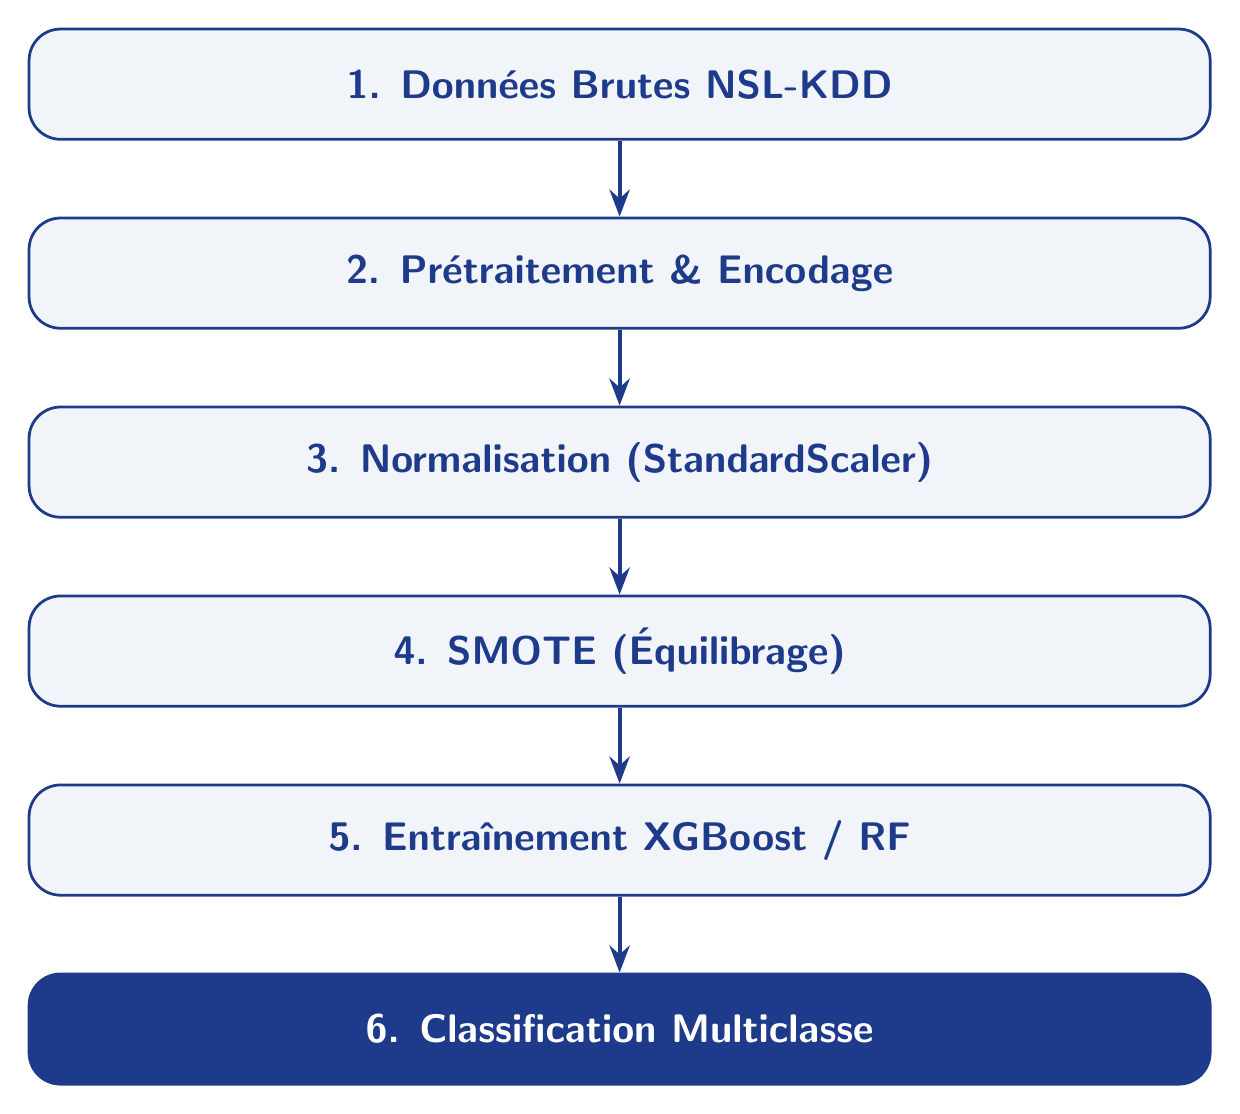
\begin{tikzpicture}[x=1mm,y=1mm]
  \tikzset{
    pnode/.style={rectangle, rounded corners=4mm,
      minimum width=150mm, minimum height=14mm,
      align=center, font=\fontsize{14}{18}\selectfont\bfseries,
      text=Primary, draw=Primary, line width=1pt, fill=HighlightBG}
  }
  
  \node[pnode] (n1) at (75,120) {1. Donn\'ees Brutes NSL-KDD};
  \node[pnode] (n2) at (75,96)  {2. Pr\'etraitement \& Encodage};
  \node[pnode] (n3) at (75,72)  {3. Normalisation (StandardScaler)};
  \node[pnode] (n4) at (75,48)  {4. SMOTE (\'Equilibrage)};
  \node[pnode] (n5) at (75,24)  {5. Entra\^inement XGBoost / RF};
  \node[pnode, fill=Primary, text=white] (n6) at (75,0)   {6. Classification Multiclasse};

  \foreach \a/\b in {n1/n2,n2/n3,n3/n4,n4/n5,n5/n6}{
    \draw[->,line width=1.5pt,Primary] (\a.south)--(\b.north);
  }
\end{tikzpicture}
\end{center}
\end{tcolorbox}

\vspace{8mm}

%% --- Box 5: Modèles & Pipeline ---
\begin{tcolorbox}[pc, title={\faCogs\; Mod\`eles \& Pipeline}]
\bodyfont\color{TextMain}

{\labelfont\color{Primary}Algorithmes ML compar\'es~:}
\vspace{2mm}

{\smallfont
\renewcommand{\arraystretch}{1.5}
\begin{tabular}{@{}p{35mm}p{115mm}@{}}
\toprule
\rowcolor{Primary}%
  \color{white}\textbf{Mod\`ele} &
  \color{white}\textbf{Caract\'eristiques} \\
\midrule
\textbf{XGBoost} & Mod\`ele de Gradient Boosting tr\`es performant pour les donn\'ees tabulaires complexes. \\
\rowcolor{HighlightBG}%
\textbf{Random Forest} & M\'ethode ensembliste bas\'ee sur le Bagging, robuste au surapprentissage. \\
\bottomrule
\end{tabular}
}

\vspace{6mm}
{\labelfont\color{Primary}Pipeline Anti-Data-Leakage~:}
\begin{itemize}[leftmargin=6mm, itemsep=2.5mm, topsep=2mm]
  \citem{Le sur-\'echantillonnage (SMOTE) est appliqu\'e \textbf{uniquement} sur le set d'entra\^inement.}
  \citem{Utilisation de \texttt{RandomizedSearchCV} combin\'e avec \texttt{StratifiedKFold} (3 folds).}
  \citem{S\'election bas\'ee sur le \textbf{Score F1 Macro}, m\'etrique optimale pour des classes fortement d\'es\'equilibr\'ees.}
\end{itemize}
\end{tcolorbox}

\vspace{8mm}

%% --- Box 6: Indicateurs Clés ---
\begin{tcolorbox}[pc, title={\faChartLine\; Indicateurs Cl\'es (KPIs)}]
\begin{center}
\vspace{4mm}
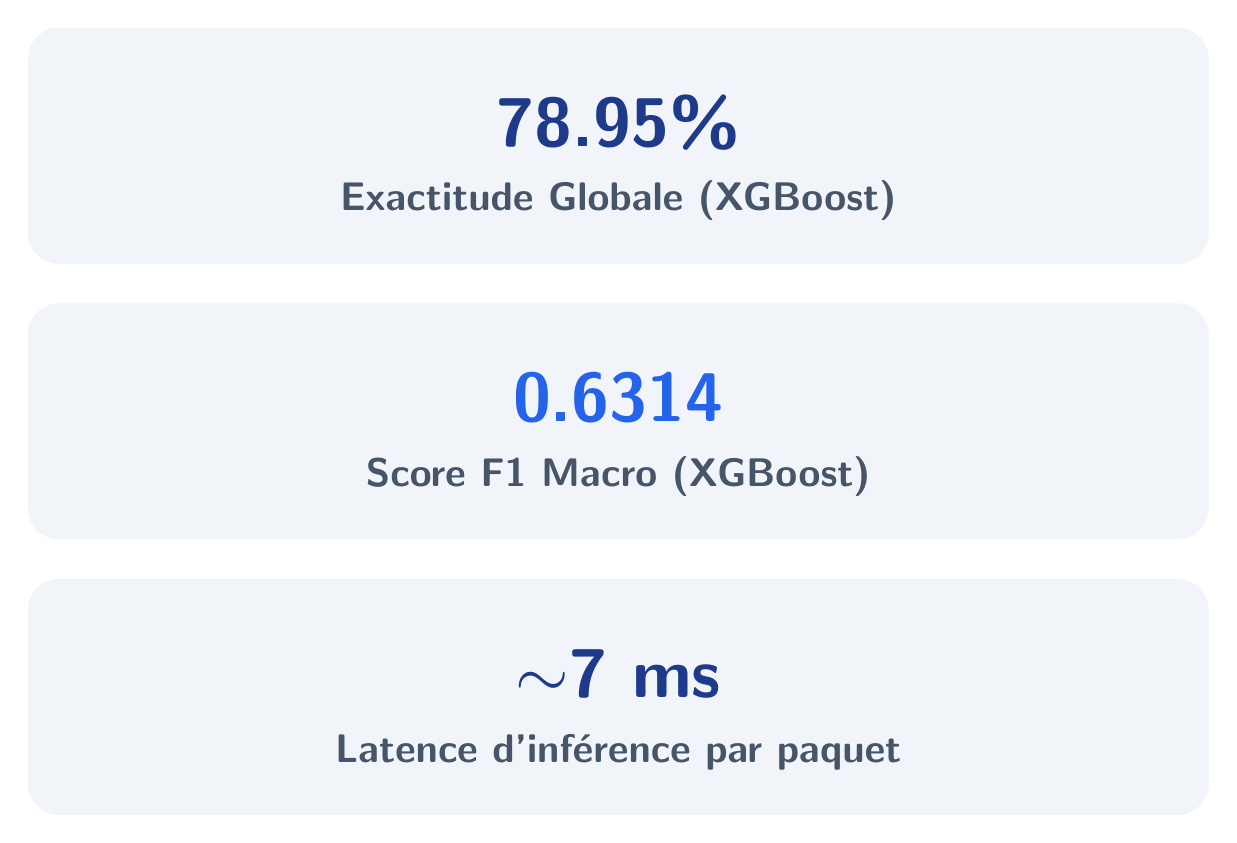
\begin{tikzpicture}[x=1mm,y=1mm]
  %% KPI 1
  \fill[HighlightBG, rounded corners=4mm] (0, 70) rectangle (150, 100);
  \node[text=Primary, font=\metricfont] at (75, 88) {78.95\%};
  \node[text=TextMuted, font=\labelfont] at (75, 78) {Exactitude Globale (XGBoost)};

  %% KPI 2
  \fill[HighlightBG, rounded corners=4mm] (0, 35) rectangle (150, 65);
  \node[text=Secondary, font=\metricfont] at (75, 53) {0.6314};
  \node[text=TextMuted, font=\labelfont] at (75, 43) {Score F1 Macro (XGBoost)};

  %% KPI 3
  \fill[HighlightBG, rounded corners=4mm] (0, 0) rectangle (150, 30);
  \node[text=Primary, font=\metricfont] at (75, 18) {$\sim$7 ms};
  \node[text=TextMuted, font=\labelfont] at (75, 8)  {Latence d'inf\'erence par paquet};
\end{tikzpicture}
\end{center}
\vspace{2mm}
\end{tcolorbox}

\end{minipage}%
\hspace{\gapW}%
%% -------------------------------------------------------------
%%  COLUMN 3
%% -------------------------------------------------------------
\begin{minipage}[t]{\colW}

%% --- Box 7: Résultats Détaillés ---
\begin{tcolorbox}[pc, title={\faTrophy\; R\'esultats D\'etaill\'es}]
\bodyfont\color{TextMain}
Les r\'esultats finaux du mod\`ele \textbf{XGBoost} sur l'ensemble de test NSL-KDD (22\,544 connexions).

\vspace{5mm}
{\labelfont\color{Primary}Rapport de Classification~:}
\vspace{2mm}

{\smallfont
\setlength{\tabcolsep}{2.5mm}
\renewcommand{\arraystretch}{1.5}
\begin{tabular}{@{}lcccc@{}}
\toprule
\rowcolor{Primary}%
  \color{white}\textbf{Classe} &
  \color{white}\textbf{Pr\'ec.} &
  \color{white}\textbf{Rappel} &
  \color{white}\textbf{F1} &
  \color{white}\textbf{Support} \\
\midrule
\textcolor{NormalColor}{\textbf{Normal}} & 97.2\% & 98.1\% & 97.6\% & 9\,711 \\
\rowcolor{HighlightBG}%
\textcolor{DosColor}{\textbf{DoS}}       & 96.6\% & 98.0\% & 97.3\% & 7\,458 \\
\textcolor{ProbeColor}{\textbf{Probe}}   & 89.4\% & 84.2\% & 86.7\% & 2\,421 \\
\rowcolor{HighlightBG}%
\textcolor{R2LColor}{\textbf{R2L}}       & 97.1\% & 21.5\% & 0.35  & 2\,887 \\
\textcolor{U2RColor}{\textbf{U2R}}       & 71.9\% & 34.4\% & 0.46  &    67 \\
\bottomrule
\end{tabular}
}

\vspace{5mm}
\bodyfont
Le mod\`ele excelle dans la d\'etection des attaques \textbf{DoS} et \textbf{Probe}. Les attaques R2L et U2R restent difficiles \`a isoler malgr\'e le SMOTE en raison de leur extr\^eme raret\'e et de leur ressemblance avec le trafic normal.
\end{tcolorbox}

\vspace{8mm}

%% --- Box 8: Interface Web ---
\begin{tcolorbox}[pc, title={\faDesktop\; Dashboard Temps R\'eel}]
\bodyfont\color{TextMain}
Nous avons d\'evelopp\'e une interface web moderne et r\'eactive pour simuler et surveiller le trafic r\'eseau en temps r\'eel.

\vspace{4mm}

\begin{center}
\begin{tikzpicture}[x=1mm,y=1mm]
  %% Outer dashed frame
  \draw[Secondary, line width=1.5pt, dashed, rounded corners=4mm]
    (0,0) rectangle (160,90);
  \fill[HighlightBG, rounded corners=4mm] (0,0) rectangle (160,90);

  %% Camera icon + label text  (centred at x=80)
  \node[text=Secondary, font=\fontsize{36}{42}\selectfont]  at (80,60) {\faCamera};
  \node[text=Primary, font=\fontsize{14}{17}\selectfont\bfseries, align=center] at (80,40)
    {Espace r\'eserv\'e pour la \\ Capture d'\'ecran de l'Interface Web};
  \node[text=TextMuted, font=\fontsize{11}{14}\selectfont, align=center] at (80,20)
    {Simulation de trafic interactif \\ \texttt{http://localhost:8000}};
\end{tikzpicture}
\end{center}

\vspace{4mm}
{\labelfont\color{Primary}Fonctionnalit\'es du Dashboard~:}
\begin{itemize}[leftmargin=6mm, itemsep=1.5mm, topsep=2mm]
  \citem{Backend robuste en \textbf{FastAPI}.}
  \citem{Pr\'ediction de flux asynchrones.}
  \citem{Visualisation des taux d'attaques en direct.}
  \citem{Solution compl\`etement conteneuris\'ee via \textbf{Docker}.}
\end{itemize}
\end{tcolorbox}

\vspace{8mm}

%% --- Box 9: Conclusion ---
\begin{tcolorbox}[pc, title={\faLightbulb\; Conclusion \& Perspectives}]
\bodyfont\color{TextMain}
Ce projet d\'emontre l'efficacit\'e de \textbf{XGBoost} pour d\'etecter les intrusions r\'eseau classiques. L'int\'egration de SMOTE a permis d'att\'enuer le d\'es\'equilibre, mais les attaques sophistiqu\'ees (U2R) n\'ecessitent des approches diff\'erentes.

\vspace{4mm}
{\labelfont\color{Primary}Perspectives d'\'evolution~:}
\begin{itemize}[leftmargin=6mm, itemsep=1.5mm, topsep=2mm]
  \citem{Utilisation de mod\`eles s\'equentiels (\textbf{LSTM}) pour capturer l'historique des paquets.}
  \citem{Mise \`a l'\'echelle sur le dataset \textbf{CICIDS2017}.}
  \citem{D\'eploiement sur mat\'eriel Edge (Edge AI).}
\end{itemize}
\end{tcolorbox}

\end{minipage}

\vspace{3mm}

%% =============================================================
%% =============================================================
%%  GRAPHS SECTION (Full Width Placeholder)
%% =============================================================
\noindent
\begin{minipage}{570mm}
\begin{tcolorbox}[pc, title={\faChartArea\; Analyses Visuelles \& Performances du Mod\`ele}]
\vspace{1mm}
\begin{center}
\begin{tikzpicture}[x=1mm,y=1mm]
  %% Placeholder Graph 1
  \draw[Secondary, line width=1.5pt, dashed, rounded corners=4mm] (0,0) rectangle (260,80);
  \fill[HighlightBG, rounded corners=4mm] (0,0) rectangle (260,80);
  \node[text=Primary, font=\fontsize{24}{28}\selectfont\bfseries] at (130,50) {\faChartBar};
  \node[text=Primary, font=\fontsize{18}{22}\selectfont\bfseries] at (130,35) {Espace Graphique 1};
  \node[text=TextMuted, font=\fontsize{14}{18}\selectfont] at (130,20) {Ins\'erer l'image du graphique ici};

  %% Placeholder Graph 2
  \begin{scope}[shift={(280,0)}]
    \draw[Secondary, line width=1.5pt, dashed, rounded corners=4mm] (0,0) rectangle (260,80);
    \fill[HighlightBG, rounded corners=4mm] (0,0) rectangle (260,80);
    \node[text=Primary, font=\fontsize{24}{28}\selectfont\bfseries] at (130,50) {\faChartLine};
    \node[text=Primary, font=\fontsize{18}{22}\selectfont\bfseries] at (130,35) {Espace Graphique 2};
    \node[text=TextMuted, font=\fontsize{14}{18}\selectfont] at (130,20) {Ins\'erer l'image du graphique ici};
  \end{scope}
\end{tikzpicture}
\end{center}
\vspace{1mm}
\end{tcolorbox}
\end{minipage}

\vspace{3mm}

%% =============================================================
%%  CONTACT SECTION (Full Width Footer with LinkedIn & QR)
%% =============================================================
\noindent

\begin{tikzpicture}[x=1mm,y=1mm]
  \fill[Primary, rounded corners=6mm] (0,0) rectangle (570,35);
  
  %% Contact 1
  \node[text=white, font=\fontsize{18}{22}\selectfont\bfseries, anchor=center] at (127.5, 23) {Sifeddine Legnioui};
  \node[text=Accent, font=\fontsize{14}{18}\selectfont, anchor=center] at (127.5, 10) {\faEnvelope\; sifeddine@email.com \quad \faLinkedin\; /in/sifeddine-legnioui};

  \draw[Accent, line width=1.5pt, dashed] (255, 5) -- (255, 30);

  %% Contact 2
  \node[text=white, font=\fontsize{18}{22}\selectfont\bfseries, anchor=center] at (382.5, 23) {Youssef Serraf};
  \node[text=Accent, font=\fontsize{14}{18}\selectfont, anchor=center] at (382.5, 10) {\faEnvelope\; youssef@email.com \quad \faLinkedin\; /in/youssef-serraf};

  \draw[Accent, line width=1.5pt, dashed] (510, 5) -- (510, 30);

  %% QR Code Placeholder
  \draw[white, line width=1.5pt, dashed, rounded corners=2mm] (520,5) rectangle (555,30);
  \fill[white!10, rounded corners=2mm] (520,5) rectangle (555,30);
  \node[text=white, font=\fontsize{20}{24}\selectfont\bfseries] at (537.5, 20) {\faQrcode};
  \node[text=Accent, font=\fontsize{8}{10}\selectfont\bfseries, align=center] at (537.5, 10) {Scan App};

\end{tikzpicture}

\end{document}
